\documentclass{article}
\usepackage[utf8]{inputenc}
\usepackage[english]{babel}
\usepackage{amsmath}
\usepackage{graphicx}
\graphicspath{{./images}}
\usepackage{amsthm}
\usepackage{mathtools}
\usepackage{marvosym}
\usepackage{mdframed}
\usepackage{mathrsfs}
\let\marvosymLightning\Lightning
\usepackage{amssymb}
\usepackage{float}
\usepackage{subfig}
\usepackage{xcolor}
\usepackage{hyperref}
\newcommand{\R}{\mathbb{R}}
\newcommand{\Z}{\mathbb{Z}}
\newcommand{\Q}{\mathbb{Q}}
\newcommand{\C}{\mathbb{C}}
\newcommand{\N}{\mathbb{N}}
\newcommand{\e}{\varepsilon}
\newcommand{\done}{\renewcommand\qedsymbol{$\blacksquare$}}
\newcommand{\contradiction}{\renewcommand\qedsymbol{$\Lightning$}}
\usepackage[left=2.54cm,right=2.54cm,top=2.54cm,bottom=2.54cm]{geometry} % page settings
\newtheorem{lemma}{Lemma}
\newtheorem{sublemma}{Lemma}[section]
% augmented matrix environment
\newenvironment{amatrix}[1]{%
  \left[\begin{array}{@{}*{#1}{c}|c@{}}
}{%
  \end{array}\right]
}
\DeclareMathOperator*{\argmax}{arg\,max}
\DeclareMathOperator*{\argmin}{arg\,min}

\hypersetup{
    citecolor=blue,
    colorlinks=true,
    linkcolor=blue,
    filecolor=magenta,      
    urlcolor=blue,
}

\title{HEB 132 Final Project Report - Opinions of Immigrants by Sex}
\author{Michael Moorman}
\date{December, 2024}
\renewcommand{\baselinestretch}{2} 

\begin{document}

\fontsize{11.8}{12}\selectfont

\maketitle

\section{Introduction}

The purpose of this project is to analyze the underlying evolutionary mechanisms that drive personal opinions regarding immigrants. In particular, we are interested in the differences in opinions between males and females, due to various relevant sex differences that may inform these opinions, such as the fact that humans are male philopatric\cite{malePhilopatry}, while females are more likely to disperse\cite{femaleDispersal}. 

This topic has been previously studied. For example, Schahbasi et al. (2021) found indeed that females were more likely to have welcoming attitudes to foreigners as opposed to males, and that this effect increased when regarding foreigners of similar ethnicity, age, and skin color\cite{immigrantOpinions}. They claim that the contradictory views of being welcoming to foreigners and xenophobia both make sense in an evolutionary context. Being accepting of foreigners can be beneficial in terms of cultural exchange and genetic diversity, both of which can bolster a group's survival, by gaining new skills, knowledge, and of course, preventing in-breeding. Similarly, although contradictory, xenophobia can also be beneficial in terms of group survival, by protecting against potential threats from outsiders.

Additionally, the authors found that this variation of opinions also has a root in simple in-group vs. out-group dynamics, as additionally noted by Tajfel et al. (1971)\cite{ingroup}. People are more likely to be accepting of those who are similar to them, and more likely to be xenophobic towards those who are different, so this effect varies quite a bit depending on the specific characteristics of the immigrant group in question. In fact, the majority of their discussion of the sex differences in these opinions cites cases of historical mass-migration of males into different areas in Europe, leading to a genetic replacement of the local male population, which could have led to a natural selection of xenophobic attitudes
in males, since those who were more xenophobic would have been more likely to survive and reproduce.

From the perspective of females, it has been noted that due to the fact that females are more likely to disperse in order to marry into other groups, it has likely been selected for that females are more friendly and accepting of strangers and foreigners, as they would have had to be in order to be accepted into a new group, as immigrants themselves\cite{femaleOpinions}. Addtionally, Wrangham (2018) noted that the violent replacement that may have led to the selection of xenophobic attitudes in males likely did not occur in females, at least not to the same extent as in males, due to the fact that females are far less likely to be attacked and killed by violent groups, but rather are more likely to be taken in as wives, which will still allow them to reproduce\cite{femaleSafety}.

In this project, we will attempt to replicate the results of Schahbasi et al. (2021) and further investigate the underlying evolutionary mechanisms that drive these opinions. However, rather than using a survey-based approach, we will use an observational approach, by analyzing the sentiment of tweets on \url{https://x.com} regarding immigrants and linking these to the sex of the author of the tweet. In this way, we hope to gain a more naturalistic view of the opinions regarding immigrants, at the slight expense of the ability to control for confounding variables. We anticipate to see similar results, in that females are more likely to have positive opinions of immigrants, while males have more xenophobic, anti-immigrant views.

\section{Methodology}

\subsection{Data Collection}

We collected a sample of 150 tweets from \url{http://x.com} that met the following conditions:
\begin{enumerate}
    \item The tweet contained the word ``immigrant'' or ``immigrants''.
    \item The tweet received less than 100 likes, in order to control for the fact that tweets with more likes are more likely to be promoted by the platform, and thus may not be representative of the general population.
    \item The tweet was unlikely to have been written by a bot, as determined by an API call to \url{https://botsentinel.com}, a website that uses machine learning to determine the likelihood that a given Twitter account is a bot in order to fight disinformation.
    \item The tweet was collected from the ``latest'' tab on the search results page, in order to ensure that the tweets were not subjet to any sort of selection bias due to the platform's algorithms.
    \item The tweet was collected from a brand new account, so that no past activity would impact the results.
\end{enumerate}

Of these 150 tweets collected, a total of 96 accounts were found with an identifiable sex of the author, based on names, profile pictures, and other information available on the account. Of these, we found that our sample comprised 74 males and 22 females. All of these resultant tweets have been saved in the following folder, for verification purposes: \url{https://drive.google.com/drive/folders/1cpWg0DbafbrTFFbc49IZHwdWZRqXhvYj?usp=sharing}. Additionally, the data and all code used to collect and analyze the data can be found in the following repository: \url{https://github.com/mjmoorman03/HEB132-Final-Project}.

\subsection{Data Analysis}
% start with how i created data set
Initially, we manually entered the tweets into a spreadsheet, with the following features:
\begin{enumerate}
    \item Male (1) or Female (0) author.
    \item The text of the tweet.
    \item Pro-immigrant (1) or anti-immigrant (0) sentinment, based on our own judgement\footnote{We acknowledge that this is a limitation of our study, but we invite the reader to verify our results by examining the tweets themselves, as we have provided a link to all tweets, and additionally to the dataset and code itself.}.
    \item Author name, either display name or handle, for linking and verification purposes.
\end{enumerate}

We loaded our data into a Pandas dataframe, and conducted the following analysis:

We employed HuggingFace's \href{https://huggingface.co/distilbert/distilbert-base-uncased-finetuned-sst-2-english?text=the+rainy+day+made+him+feel+quite+down}{default sentiment analysis model}, which is a pre-trained machine learning model that can classify the sentiment of a given text as positive or negative. We used this model to classify the sentiment of the tweets, in order to verify our own judgements. However, we found that the model was not very accurate to our own judgement. These tweets largely exist in an argumentative context, and the sentiment of the text can be quite negative even if the position is to defend immigrants, as it could be attacking the one it responds to. Similarly, many individuals are deeply enthusiastic about deporting immigrants, and thus their sentiment can be quite positive, despite the fact that they are expressing a negative opinion, even with hateful language. So, we have decided to continue with our own judgement, as truthfully, there exists no language model that can classify human intention as well as a human can. We discuss this limitation further in the discussion section.

Then, we simply split the data into two groups, based on the sex of the author, and calculated the contigency table of the number of pro-immigrant and anti-immigrant tweets for each group. We then conducted a chi-squared test of independence to determine if the difference in opinions between males and females was statistically significant.

We present these results below.

\section{Results}

Our contigency table is as follows:

\begin{figure}[H]
\begin{table}[H]
    \centering
    \begin{tabular}{|c|c|c|}
    \hline
    & Pro-Immigrant & Anti-Immigrant \\ 
    \hline
    Male & 18 & 56 \\ \hline
    Females & 14 & 8 \\
    \hline
    \end{tabular}
    \caption{Contigency Table of Opinions by Sex}
    \label{tab:contigency}
\end{table}
\end{figure}
\vspace{-0.5cm}
Already, it is quite clear that there is a significant difference in opinions between males and females regarding immigrants. To see this more clearly, see figure \ref{fig:piePlots}.

\begin{figure}[H]
    \centering
    \subfloat
    {
        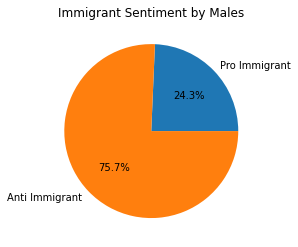
\includegraphics[width=0.34\textwidth]{males.png}
    }
    \subfloat
    {
        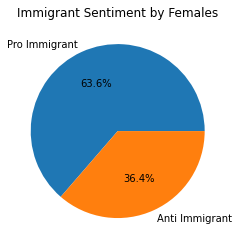
\includegraphics[width=0.27\textwidth]{females.png}
    }
    \caption{Pie Charts of Opinions by Sex}
    \label{fig:piePlots}
\end{figure}

We then conducted a Pearson's chi-squared test of independence, with the following hypotheses:
\begin{align*}
    H_0 &: \text{There is no difference in opinions between males and females with regard to immigrants.} \\
    H_1 &: \text{There is a difference in opinions between males and females with regard to immigrants.}
\end{align*}

We found that the test statistic was $\chi^2 = 10.\overline{09}$, with 1 degree of freedom, and a p-value of $0.00149$. Thus, we reject the null hypothesis, and conclude that there is a significant difference in opinions between males and females. 

However, to be certain, we also used a Fisher's exact test, which is more appropriate for small sample sizes, and found that the p-value was $0.00147$, which is very close to the p-value of the chi-squared test. Thus, we can be confident in our results, and indeed include that we have found a statistically significant difference in opinions between males and females regarding immigrants, and, barring the limitations discussed below, this can be taken as evidence that our results are generalizable to the population at large.

\section{Discussion}

Our results are consistent with the findings of Schahbasi et al. (2021), in that we found that females were more likely to have positive opinions of immigrants, while males were more likely to have negative opinions. This is consistent with the evolutionary mechanisms that we discussed in the introduction, such as the fact that humans are male-philopatric, and thus females are more likely to be accepting of strangers and foreigners, as they would have had to be in order to be accepted into a new group themselves upon dispersal. Additionally, males are quite unlikely to be willing to accept strangers into their group, as again, they are male-philopatric, and thus generally have established social structures that they would not want immigrants to disrupt.

Indeed, this similarly agrees with the other evolutionary mechanisms that we discussed, such as the proposed explanation of male xenophobia as a result of historical mass-migration of males into different areas in Europe, leading to a genetic replacement of the local male population and thus a natural selection of xenophobic attitudes in males, but not in females. This is consistent with our results, as shown above.

To further explain the reason for this difference in opinions, we can consider the general contexts behind the tweets. For example, many of the tweets that we classified as anti-immigrant dealt with the large influx of immigrants through the southern border of the United States. Many individuals advocated for the mass deportation of such immigrants, and as a United States citizen, this isn't necessarily an unreasonable opinion to have, as long as one is optimizing specifically for their ability to produce successful offspring. Proximally, one may believe that these immigrants are disproportionally violent\footnote{This is an idea repeatedly presented in these tweets, but is largely not supported by the data.}, and of course, one would be xenophobic towards those who are violent, as it is a threat to one's own survival, and the survival of one's offspring. More distally, one could consider the resources in the United States as a fixed pool, and thus the more individuals that are in the pool, the less resources there are for one's own offspring. And since immigrants are less likely to be related to oneself than those who are already in the pool, it is not unreasonable to be xenophobic towards them, as they are a threat to one's own reproductive success, genetically speaking. These are perhaps the reasons we see a significant baseline of anti-immigrant rhetoric in both of our independent variable groups. 

Then, we consider why, for males, the rate of anti-immigrant opinion is so much higher. Proximally, it could be for reasons of social status, as male philopatric groups are more likely to have established social structures that they would not want broken. Indeed, if our social structures were rigid, and all those in the United States were offspring of others in the United States, then the only source of a confounder to one's own status would be an immigrant. Thus, it would make sense, given the significantly smaller population size of early human groups, that males would be more likely to be xenophobic, as their social status would be more likely to be threatened by an immigrant. On a larger scale, this may play a role, so indeed, holding xenophobic attitudes may indeed increase a male's reproductive success, as it would protect his social status, and thus his ability to produce offspring. 

Then, we consider the female perspective. Pro-immigrant opinions are likely to increase a female's reproductive success, as it would increase the genetic diversity of the group, which is typically a female's concern, and also because it is important for a female to be able to disperse in the first place. Of course, there are also benefits to being accepting of immigrants, such as cultural exchange and genetic diversity, so it stands to reason that females would be more likely to be accepting of immigrants than males would.

\subsection{Limitations}
% reliability of judgement of sentiment
% do make the argument that while this is not an objective measure, it is still far more valid that something like counting a smile as a signifier as happiness, since we are able to understand the context of the tweet and the intention of the author, and any reasonably intelligent human would come up with the same classification as we did, given the same context. It is not as though we are making a subjective judgement, but rather an objective one, only that it is not based on a simple rule, but rather a complex understanding of the context of the tweet.

% potential bots in the dataset

% potential misclassification of sex, although only if individuals are misrepresenting themselves

There are a number of limitations to our study. Firstly, our classification of the opinion in the tweets is not based on a particularly objective measure, as it is based on our own judgement. However, we believe that this is a reasonable measure, as the intention behind a tweet is indeed objective, and we posit that with the context of each tweet present, which we have provided, any reasonably truthful human would come to the same conclusions as we did. Indeed, our sentiment analysis via HuggingFace's model was not particularly accurate, but this is not a particularly impactful drawback, as truthfully, there is no language model that can classify human intention as well as a human can. We invite the reader to verify our results by examining the tweets themselves, as we have provided a link to all tweets, and additionally to the dataset and code itself.

Additionally, there is the potential for bots to be present in our dataset, as the bot detection tool that we used is not perfect. In addition, our designation of sexes is also susceptible to error, as individuals may misrepresent themselves online, but we believe that this is unlikely to be a significant issue, as the number of individuals who would do so is likely to be quite small, and the number of bots who would be able to pass the bot detection tool is also likely to be quite small.

There is also a potential issue with our findings regarding the fact that certain populations may be more likely to be outspoken about their beliefs one way or another. For example, it is possible that anti-immigrant males are more likely to be outspoken about their beliefs than anti-immigrant females for some reason, and there could therefore be a self-selection issue in our sample, as we can't quite compare males and females 1-to-1 due to various other differences between the sexes. However, we believe that willingness to be outspoken about one's beliefs is a rather good proxy for one's beliefs, and thus we believe that this is not a significant issue.
\subsection{Future Directions}

This project could be expanded in a number of ways. Firstly, it would be great to get a larger sample of tweets, in order to increase the power of our study, despite the very low p-value that we found. In addition to this, it would be beneficial to separate the tweets by country, in order to contextualize our results, and perhaps draw conclusions about different types of immigration and how they affect opinions between males and females.

More than strictly changing our approach, it would be beneficial to have a sentiment analysis model that has been pre-trained or fine-tuned on tweets and even potentially on immigration-related tweets, such that it is able to distinguish between positive and negative opinions about immigrants, rather than strictly positive and negative sentiment. This would allow us to more accurately classify the sentiment of the tweets, and to do so in an objective manner, which would be beneficial for the generalizability of our results.

\section{Conclusion}

This study reinforces the hypothesis that evolutionary mechanisms influence the differences in male and female opinions toward immigrants. Females, more predisposed to dispersal and integrating into new groups, displayed greater acceptance of immigrants, while males, shaped by evolutionary pressures favoring territoriality and in-group protection, were more likely to express xenophobic views.

Although our methodology had limitations, our findings align with prior studies, offering a nuanced and modern perspective on how evolutionary factors and social contexts interact to shape opinions. This work highlights the importance of understanding these dynamics in broader discussions of migration and policy. Future research should aim to refine and expand these analyses, potentially leveraging advancements in machine learning and larger datasets to build upon our findings.

\section{Data Appendix}
Due to the text of the tweets being quite long, we have provided a link to the repository containing the dataset, as well as a link to the folder containing the tweets themselves in the Methodology section of this paper, in lieu of providing the dataset in this paper.

\begin{thebibliography}{6}
    \bibitem{malePhilopatry} Milich K. M. (2024). Male-philopatric nonhuman primates and their potential role in understanding the evolution of human sociality. Evolutionary anthropology, 33(1), e22014. \url{https://doi.org/10.1002/evan.22014}

    \bibitem{femaleDispersal} Nichols, H. J., Zecherle, L., \& Arbuckle, K. (2016). Patterns of philopatry and longevity contribute to the evolution of post-reproductive lifespan in mammals. Biology letters, 12(2), 20150992. \url{https://doi.org/10.1098/rsbl.2015.0992}

    \bibitem{immigrantOpinions} Schahbasi, A., Huber, S., \& Fieder, M. (2021). Factors affecting attitudes toward migrants-An evolutionary approach. American journal of human biology : the official journal of the Human Biology Council, 33(1), e23435. \url{https://doi.org/10.1002/ajhb.23435}

    \bibitem{ingroup} Tajfel, H., Billig, M., Bundy, R., \& Flament, C. (1971). Social categorization in intergroup behavior. European Journal of Social Psychology, 1, 149-178.

    \bibitem{femaleOpinions} Towner, M. C. (2002). Linking dispersal and marriage in humans: Life history data from Oakham, Massachusetts, USA (1750-1850). Evolution and Human Behavior, 23(5), 337-357.

    \bibitem{femaleSafety} Wrangham, R. W. (2018). Two types of aggression in human evolution. Proceedings of the National Academy of Sciences, 115(2), 245-253.

\end{thebibliography}

\end{document}